\documentclass[12pt]{article}
\usepackage[utf8]{inputenc}
\usepackage{parskip}
\usepackage[spanish]{babel}
\usepackage{amsmath, amssymb}
\usepackage{graphicx}
\usepackage{makecell}
\usepackage{geometry}
\usepackage{caption}
\usepackage{float}
\usepackage[hidelinks]{hyperref}


% --------------------- Comandos para pie de página ---------------------
\usepackage[backend=biber, style=apa]{biblatex}
\addbibresource{referencias.bib}
\usepackage{hyperref}
\usepackage{url}
\usepackage{csquotes}

\makeatletter
\g@addto@macro{\UrlBreaks}{\UrlOrds}
\makeatother

\renewcommand{\footnoterule}{%
  \kern -3pt                         % Espacio vertical sobre la línea
  \hrule width \textwidth height 0.4pt % Ancho total de la página y grosor
  \kern 2.6pt                        % Espacio vertical debajo de la línea
}
% -----------------------------------------------------------------------

\addbibresource{referencias.bib}
\geometry{letterpaper, margin=2.5cm}
\setlength{\parskip}{1em}

\begin{document}
\begin{titlepage}
\begin{center}
    % Logos
    \begin{minipage}{0.3\textwidth}
        
\includegraphics[width=0.8\linewidth]{imagenes/UNAM_Logo.png}
    \end{minipage}\hfill
    \begin{minipage}{0.4\textwidth}
        \begin{center}
            \textbf{\Large Universidad Nacional Autónoma de México}\\[0.2cm]
            \textbf{Facultad de Ciencias}\\[0.2cm]
        \textbf{Bases de Datos}
        \end{center}
    \end{minipage}\hfill
    \begin{minipage}{0.3\textwidth}
        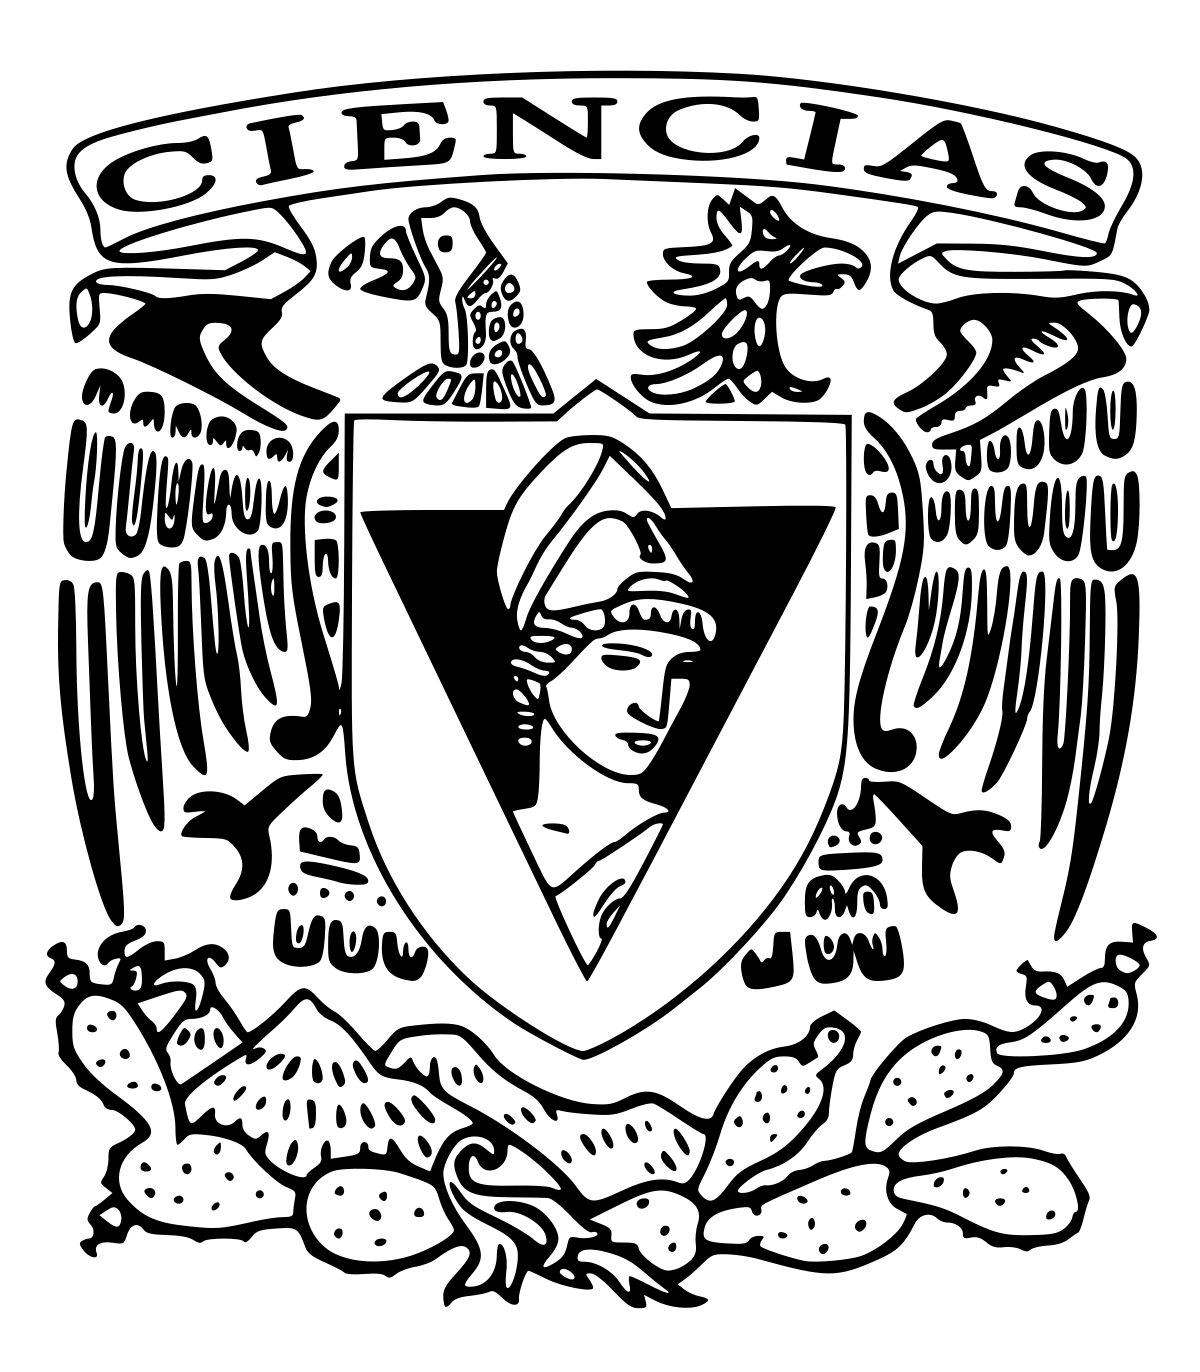
\includegraphics[width=0.8\linewidth]{imagenes/Logo_FC.png}
    \end{minipage}
    \vspace{3cm}
    \textbf{\large Tarea 2}\\
    Licenciatura en Ciencias de la Computación\\
    Profesor: Gerardo Avilés Rosas \\
    \vspace{2cm}
    \textbf{Integrantes: }\\
    Cisneros Tenorio Diego Alexander\\
    Nuñez Ruiz José Manuel \\
    Olmos Ortiz Andrea Lucia\\
    Reynoso Ascencio Alexa \\
    Vega Navas Saúl \\
    \vspace{2cm}
    \textbf{Fecha de entrega: } 22 de septiembre del 2026
    \vfill
\end{center}
\end{titlepage}
\tableofcontents
\newpage

% Preguntas

 \section{Conceptos del Modelo Entidad – Relación}
\subsection*{a. }

\addcontentsline{toc}{subsection}{d.}
    
\textbf{¿Qué es un tipo de relación? Explica las diferencias con respecto a una instancia de relación.}

Primero, una relación es una asociación entre entidades, la cual cuenta con un grado y restricciones de cardinalidad y participación. Un tipo de relación es un subconjunto del producto cartesiano de n-Entidades (por ejemplo, la relación binaria es un subconjunto del producto cartesiano de la entidad A y la entidad B). También la podemos definir como el conjunto de todas las instancias de relación, y precisamente este último punto es la clave sobre cómo diferenciar una instancia de relación y un tipo de relación: una instancia es un elemento en particular del tipo de relación. Por ejemplo, si tenemos la relación binaria Estudiar entre Alumno y Materia, el conjunto de todas las instancias de la relación forman el tipo de relación, mientras que Juanito que estudia Matemáticas es una instancia particular de la relación, donde Juanito forma parte del conjunto de entidades de Alumno y Matemáticas forma parte del conjunto de entidades de Materia.

 \subsection*{b. }

\addcontentsline{toc}{subsection}{b.}
\textbf{¿Bajo qué condiciones se puede migrar un atributo de algún tipo de entidad que participa en un tipo de relación binaria y convertirse en un atributo del tipo de relación? ¿Cuál sería en el efecto?}\\ \\
Podemos migrar un atributo a una relación cuando su valor depende de la combinación de instancias las entidades, es decir, que el atributo no describe una propiedad intrínseca de una de las entidades, sino una característica de esa asociación en particular.\\ \\
Hacer esto puede generar la pérdida del acceso directo al atributo. Después de migrar el atributo, este pertenece a la relación entre las dos entidades, por lo que para consultarlo es necesario identificar ambas partes de la relación. Mientras que antes de migrar el atributo solo consultaríamos directamente su entidad.
 \subsection*{c. }

\addcontentsline{toc}{subsection}{c.}
    
\textbf{¿Cuál es el significado de un tipo de relación recursiva? Proporciona un par de ejemplos de este tipo de relación.}

Una relación recursiva es un tipo de asociación de una entidad consigo misma, es decir, es un tipo de relación con grado 1 (unaria).  A continuación algunos ejemplos.
\begin{enumerate}
\item Supongamos que tenemos una situación deportiva en la que se trata de modelar:
  \begin{itemize}
  \item En cada entrenamiento, cada jugador es acompañado por otro jugador y cada jugador solo puede tener un compañero.
  \end{itemize}
  En este caso tenemos la relación acompañar, que está situada sobre una única entidad, la entidad jugador. De este modo, es posible plantear la relación como una relación unaria, en la que un jugador esté relacionado con otro jugador bajo la relación acompañar (con cardinalidad 1:1).
  
\item Supongamos que tenemos una situación en la que queremos almacenar información sobre los lenguajes de programación y queremos modelar:
  \begin{itemize}
  \item Cada lenguaje de programación es construido a su vez por otro lenguaje de programación.
  \end{itemize}
  En esta situación, es posible plantear un modelo usando la entidad Lenguaje que está asociada consigo misma bajo la relación construir (con cardinalidad 1:1).
  
\item Supongamos que tenemos una situación en la que queremos almacenar datos sobre el plan de estudios de una carrera y queremos modelar:
  \begin{itemize}        
  \item En un curso, hay materias que preceden a otras.                
  \end{itemize}
  Para este caso, se puede plantear un modelo usando la entidad Materia que está asociada consigo misma bajo la relación preceder (con cardinalidad N:M).
  
\item Supongamos que tenemos una situación en la que queremos almacenar datos sobre personas en un grupo.
  \begin{itemize}
  \item En un grupo, hay personas que conocen a otras personas.            
  \end{itemize}
  Para este caso, se puede plantear un modelo usando la entidad Persona que está asociada consigo misma bajo la relación conocer (con cardinalidad N:M).
  \end{enumerate}

 \subsection*{d. }

\addcontentsline{toc}{subsection}{d.}
    
\textbf{Responde a las siguientes cuestiones, deberás indicar si son posibles o no, justificando tu respuesta.}

\textbf{¿Un atributo compuesto puede ser llave?}

\textbf{R.} Sí puede ser, y su unicidad es distinguible por los `sub-atributos' que lo integran.

\textbf{¿Un atributo multivaluado puede ser llave?}

\textbf{R.} En teoría sí, pero esto no solo restringe la cantidad de datos almacenable en dicho atributo (para mantener la inmutabilidad de la llave), sino que también rompe con las reglas más fundamentales de normalización de bases de datos, ya que la Primera Forma Normal indica registrar valores atómicos por cada columna.

En caso de que existan valores que dependan exclusivamente de una agrupación de datos en particular, es mejor describir por aparte una relación entre éstos y el único valor dependiente.
\begin{itemize}
    \item Un ejemplo se da si se quiere almacenar una entidad \textit{Promoción} de la que sus características dependen de los productos almacenados, es mejor que éstas se relacionen de forma 1:$N$ con la entidad \textit{Producto} en lugar de poner la lista como llave.
\end{itemize}


\textbf{¿Un atributo derivado puede ser llave?}

\textbf{R.} En teoría sí pero bajo restricciones de unicidad de los atributos base, no obstante, esto no supone una implementación viable puesto que, por naturaleza, los atributos derivados no siempre son persistentes, además de que genera una dependencia de la llave $-$y por consecuencia, de la entidad$-$ en un atributo no llave.

\textbf{¿Un atributo multivaluado puede ser compuesto?}

\textbf{R.} Sí, puede ser; por ejemplo, si se guarda el historial de un trabajador, se pueden llegar a almacenar varias agrupaciones de datos como el grado y la institución, pues un trabajador pudo haber tenido varios empleos.

\textbf{¿Un atributo multivaluado puede ser derivado?}

\textbf{R.} Sí, se puede dar, por ejemplo, a partir de operar sobre otro atributo multivaluado, como en una filtración de datos.
\begin{itemize}
    \item Un caso puede darse si, al guardar información de proyectos de un departamento, se calculan y almacenan aquellos que están vigentes.
\end{itemize}

\textbf{¿Qué implicaría la existencia de una entidad cuyos atributos sean todos derivados?}

\textbf{R.} Esto implica que todos sus datos son calculados a partir de otras fuentes en el sistema, por lo que o es una implementación redundante o se trata de información derivada de una consulta. Además, por la volatilidad comentada en previamente, esta entidad no puede tener una llave con la que dar paso a una integridad referencial fiable.
 \subsection*{e. }

\addcontentsline{toc}{subsection}{e.}
    
\textbf{Explica el concepto de categorías (herencia múltiple) en el modelo E-R y proporciona dos ejemplos de la vida real en donde se aplique este concepto.}

Una \textbf{categoría} se utiliza en el modelo E-R extendido para representar la unión de dos o más superclases que pertenecen a distintos tipos de entidades. Las superclases de una categoría suelen tener atributos y llaves primarias completamente diferentes entre sí. Por lo que, cuando las llaves son distintas, recurrimos a una llave sustituta para identificar de manera única a los elementos de la categoría. En este modelo, una entidad de la categoría pertenece a una sola de las superclases a la vez, por lo que la herencia de atributos es selectiva.

Una categoría es diferente de la \textbf{herencia múltiple}. En la herencia múltiple, la subclase hereda simultáneamente de varias superclases que comparten el mismo atributo llave; mientras que en una categoría, la subclase representa la unión de clases de distintos tipos con llaves diferentes.

\textbf{Ejemplos de la vida real:}

\begin{enumerate}
    \item \textbf{Emisión de factura :} Para emitir un comprobante fiscal podemos tener distintos tipos de personas, puede ser una \texttt{PersonaFísica} (identificada por CURP), una \texttt{Persona moral} (identificada por RFC) o un \texttt{Extranjero} (identificado por su RFC genérico extranjero). Como las tres superclases tienen llaves distintas, \texttt{Cliente} se modela como una categoría con un \texttt{IdCliente} como llave sustituta.
    
    \item \textbf{Registro de Pago Electrónico:} En una tienda en línea podemos realizar el pago de un producto de distintas maneras; ya sea mediante \texttt{TarjetaDeCrédito} (identificada por el número de tarjeta), una \texttt{CuentaBancaria} (identificada por la CLABE) o un \texttt{Deposito} (identificado por el número de transacción). La categoría \texttt{MétodoDePago} unifica estas distintas entidades para asociarlas a una orden de compra mediante un \texttt{IdMetodoPago} como llave sustituta.
\end{enumerate}

 \section{Entendiendo el Modelo Entidad – Relación}
\subsection*{i. }

\addcontentsline{toc}{subsection}{d.}
\textbf{A continuación, se muestran tres representaciones posibles referidas a las relaciones entre Sitios de taxis, Choferes y Taxis. Analiza las ventajas y desventajas de cada propuesta, contestando las preguntas que se presentan a continuación:}
\begin{enumerate}
    \item \textbf{Indica qué diagramas representan la información requerida por las siguientes solicitudes de información:}

    \textbf{¿Qué taxis maneja el chofer Raúl López en el sitio Santa Fe?}

    El diagrama a) no puede contestar satisfactoriamente esta consulta, pues aunque un chofer puede tener un taxi en un sitio, no sabemos si el chofer lo maneja; por ejemplo, podemos saber que Raúl López tiene un taxi rojo en el sitio Santa Fe, pero no sabemos si lo maneja él. Por otro lado, el diagrama b) tampoco lo puede satisfacer, pues sabes qué chofer maneja qué taxi, pero no sabes si lo maneja en ese sitio; solo sabes que el taxi tiene sitio, pero no si lo maneja allí; por ejemplo, el chofer Raúl López maneja un carro rojo y ese carro rojo tiene sitio en Santa Fe, pero no sabemos si Raúl López lo maneja en Santa Fe. Finalmente, el diagrama c) sí lo satisface, pues precisamente la agregación asocia a cada chofer con la relación Manejar a un par exacto (Sitio, Taxi). Así, si Raúl López maneja un taxi (digamos rojo) que pertenece al sitio Santa Fe, como el par ya está hecho como un todo, se sabe que es en ese sitio específico.

    \textbf{¿A qué sitios está afiliado el chofer Carlos Reyes?}

    Claramente el diagrama a) lo satisface, pues te permite asociar a cada chofer con un sitio y un taxi mediante la relación Tener, así que podemos conocer a qué sitios está asociado el conductor Carlos Reyes. Sin embargo, ni el diagrama b) ni el c) satisfacen conocer a qué sitio está afiliado. En el diagrama b), Carlos Reyes puede manejar el taxi rojo y ese taxi tiene sitio, pero al carecer de una relación directa entre chofer y sitio, no se sabe si Carlos Reyes tiene sitio (o está afiliado) de forma independiente. Asimismo, en el diagrama c), un chofer maneja un par (Sitio, Taxi); sin embargo, si el chofer no maneja activamente, no sabemos si está asociado al sitio o no.

    \textbf{¿Qué taxis están asociados al sitio Universidad?}

    En este caso, los 3 diagramas me pueden dar a conocer qué taxis están asociados al sitio Universidad, ya que todos cuentan con la relación Tener, la cual asocia directamente a la entidad Taxi con la entidad Sitio. Así, resta encontrar las parejas que tengan en la posición de sitio a Universidad y un taxi distinto en cada uno (se puede notar que el diagrama a) causa un poco de redundancia, pues además asocia al chofer con ellos, cosa que trae repeticiones en las parejas de Taxi y Sitio).

    \item \textbf{¿Qué modificación harías en el diagrama de la figura a), sin perder información, para que se puedan conocer qué taxis maneja cada chofer?}

    En este caso, para no perder información, es suficiente agregar una relación binaria directa entre Chofer y Taxi llamada Manejar y mantener la relación Tener. Con ello podríamos saber además qué chofer maneja qué taxi. El diagrama se muestra en la siguiente figura:
    \begin{figure}[H]
        \centering
        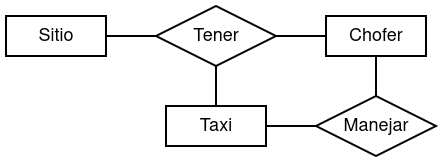
\includegraphics[width=0.6\textwidth]{imagenes/a)manejar.png}
        \caption{Diagrama actualizado con la relación Manejar.}
    \end{figure}

    \item \textbf{¿Qué diferencia existe entre los diagramas de las figuras a) y c)?}

    La diferencia más obvia a primera vista, como se notó en la primera pregunta, es que el diagrama a) no nos permite saber qué chofer maneja qué taxi, mientras que el diagrama c) sí lo hace. Sin embargo, la distinción estructural más relevante es que el inciso a) ubica a todas las entidades al mismo nivel, por lo que aun si pudiera asociar a un taxi y un chofer, no da información al mismo tiempo sobre en qué sitio lo maneja; mientras que el diagrama c) utiliza la abstracción de agregación para empaquetar el par (Sitio, Taxi). Esto nos permite conocer qué chofer maneja un taxi en un sitio determinado.

    \item \textbf{Cómo modificarías el diagrama de la figura a) para representar las siguientes restricciones:}

    \textbf{Nota: Para facilitar la resolución del problema y con la aprobación de uno de mis ayudantes, asumiré que en el inciso a) la relación Tener también funciona como Manejar.}

    \textbf{Un chofer no puede manejar más de un taxi en el mismo sitio.} 

    Esta es una restricción de cardinalidad. Si agregamos una restricción de cardinalidad máxima de uno apuntando hacia Taxi (es decir, cambiamos la línea recta por una flecha desde la relación Tener hacia Taxi), logramos que cada chofer pueda estar en varios sitios, pero solo maneje un taxi. De esta forma, un chofer podría cambiar de sitio y poder manejar el mismo taxi u otro distinto.

    \textbf{Un taxi no puede ser manejado por más de un chofer en el mismo sitio.}

    Similarmente, ahora necesitamos crear una restricción de cardinalidad máxima apuntando hacia Chofer. Cambiamos la línea recta por una flecha desde la relación Tener hacia Chofer. Así, cada taxi podría estar en muchos sitios, pero solo tendría un chofer asignado a la vez, y tendría que cambiar de sitio para ser manejado por otro.

    \textbf{El siguiente diagrama representa ambas restricciones aplicadas al diagrama a):}
    \begin{figure}[H]
        \centering
        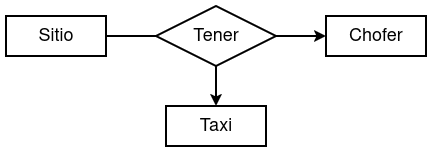
\includegraphics[width=0.6\textwidth]{imagenes/a)Restricciones.png}
        \caption{Diagrama actualizado con las restricciones correspondientes.}
    \end{figure}
\end{enumerate}

 \subsection*{2.ii}

El siguiente \textbf{modelo E-R corresponde} a una base de datos de \textbf{una universidad}. Luego de unos años de funcionamiento, se han detectado una \textbf{serie de deficiencias en el sistema de mantenimiento} de datos y se quieren realizar las \textbf{siguientes modificaciones}:
\begin{figure}[H]
    \centering
    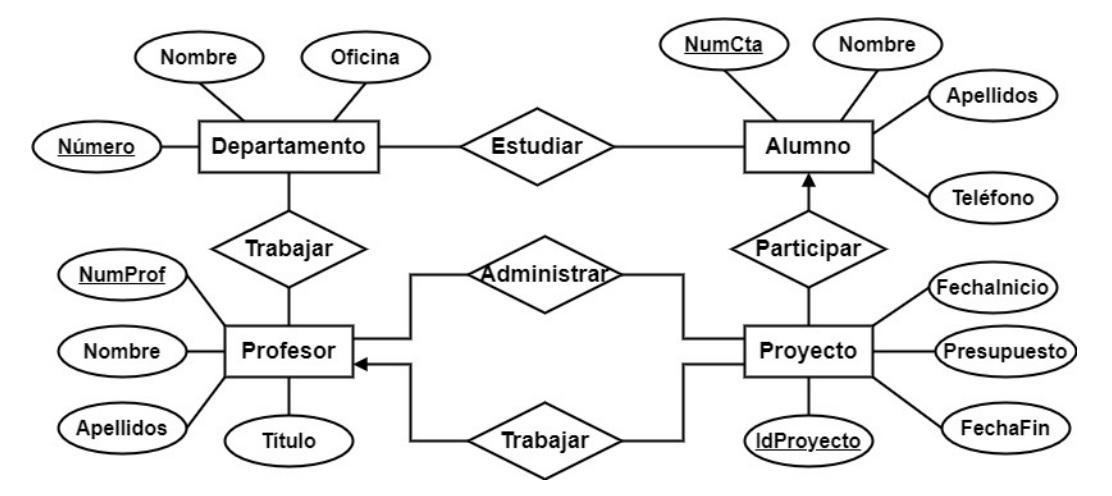
\includegraphics[width=1\linewidth]{imagenes/ModeloOriginal.png}
\end{figure}
\begin{itemize}
    \item Dado que solo los alumnos graduados pueden participar en proyectos, se desea distinguir entre alumnos graduados y no graduados. Además de la información almacenada para un alumno, para los alumnos graduados se desea almacenar el título que posee y para los alumnos no graduados su número de expediente.
    \item Un alumno graduado puede ser tutor de varios alumnos no graduados y cada alumno no graduado tendrá solamente un tutor.
    \item Se desea almacenar, para cada profesor, el nombre del cargo que ocupa en cada departamento (el cual es único dentro del departamento) y la carga horaria asociada. Un mismo cargo puede tener diferente carga horaria dependiendo del departamento y/o del profesor. Dentro de un departamento no pueden existir profesores con el mismo cargo. Un profesor podrá tener el mismo cargo en varios departamentos.
    \item Cuando un alumno graduado participa en un proyecto y un profesor debe supervisar su trabajo en ese proyecto. Cada alumno graduado podrá trabajar en múltiples proyectos, en los cuales podrá ser supervisado por diferentes profesores.
\end{itemize}
\textbf{Obtén un nuevo modelo E-R modificando el modelo presentado, para incorporar los cambios deseados. Identifica las restricciones de cardinalidad, participación e identidad en el nuevo modelo propuesto.}\\ 
\begin{figure}[H]
        \centering
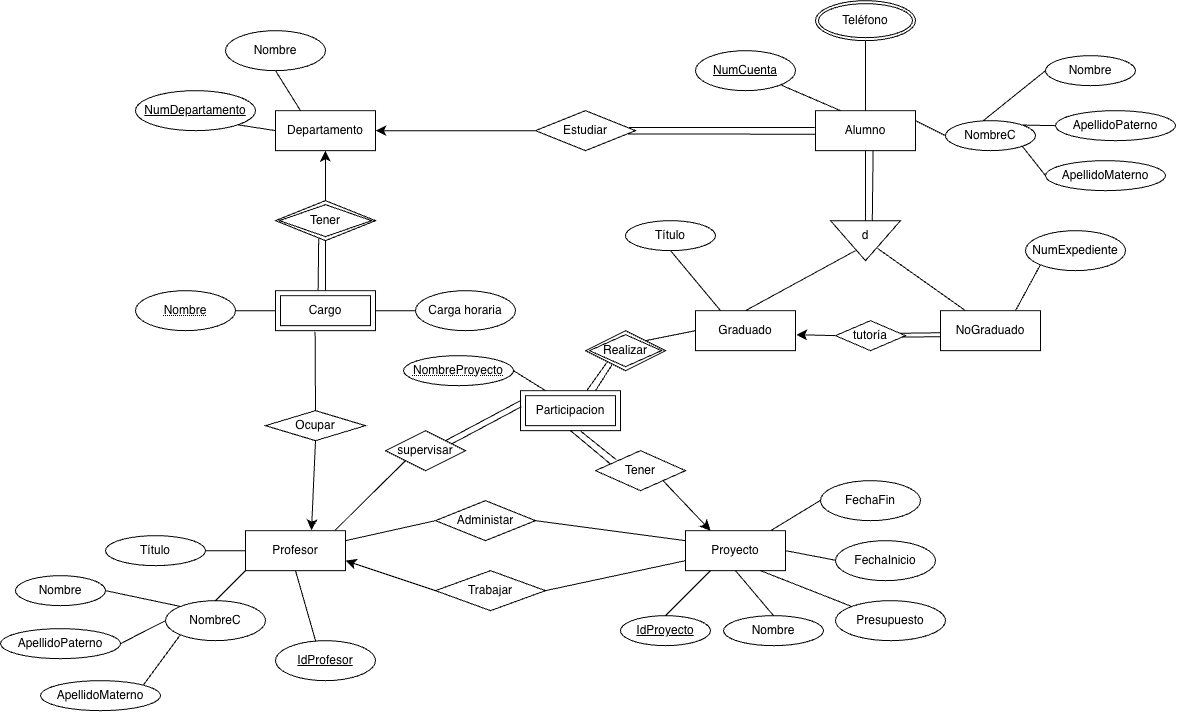
\includegraphics[width=1.1\linewidth]{imagenes/ModeloModificado.png}
    \end{figure}

\subsubsection*{Entidades:}
\begin{itemize}
    \item Profesor
    \item Departamento
    \item Proyecto
    \item Participación(Débil)
    \item Cargo(Débil)
    \item Alumno (SuperEntidad)
    \begin{itemize}
        \item Graduado
        \item No Graduado
    \end{itemize}
\end{itemize}
\subsubsection*{Atributos:}
\textbf{Profesor}
\begin{itemize}
    \item Titulo
    \item Nombre Completo(Nombre,Paterno,Materno)
    \item IdProfesor(identificador)
\end{itemize}
\textbf{Departamento}
\begin{itemize}
    \item Nombre 
    \item Número de Departamento(identificador)
\end{itemize}
\textbf{Proyecto}
\begin{itemize}
    \item Fecha de Inicio
    \item Fecha de Fin
    \item Presupuesto
    \item IdProyecto(identificador)
\end{itemize}
\textbf{Participación}
\begin{itemize}
    \item Nombre del proyecto(discriminante)
\end{itemize}
\textbf{Cargo}
\begin{itemize}
    \item Nombre del cargo(discriminante)
    \item carga horaria
\end{itemize}
\textbf{Alumno}
\begin{itemize}
    \item Telefono(multivaluado)
    \item Nombre Completo (Nombre,Paterno,Materno)
    \item Número de cuenta (identificador)
\end{itemize}
\textbf{Graduado}
\begin{itemize}
    \item Titulo
\end{itemize}
\textbf{No Graduado}
\begin{itemize}
    \item Número de expediente
\end{itemize}

\subsubsection*{Relaciones:}
\begin{itemize}
    \item \textbf{Estudiar} Departamento-Alumno \textbf{1:N}\\ \\
    Departamento: Parcial(0,N)\\
    Alumno:Total(1,1)\\ \\
    Muchos alumnos estudian en un  departamento. \\ \\
    Un alumno necesita estudiar en un departamento. \\
     
    \item \textbf{Tutoria} Graduado-NoGraduado \textbf{1:N}\\ \\
    Graduado:Parcial(0,N)\\
    No Graduado:Total(1,1)\\ \\
    Un alumno graduado puede ser tutor de varios alumnos no graduados. \\ \\
    Los alumnos no graduados solo tienen 1 tutor.

    \item \textbf{Realizar} Graduado-Participación \textbf{1:N}\\ \\
    Graduado:Parcial(0,N)\\
    Participación:Total(1,1)\\

    Los alumos pueden realizar varias participaciones en distintos proyectos.\\ \\
    Una participacion requiere necesariamente un alumno

\item \textbf{Tener} Proyecto-Participación \textbf{1:N}\\ \\
    Proyecto:Parcial(0,N)\\
    Participación:Total(1,1)\\ \\
    Una participación requiere necesariamente un proyecto.\\ \\
    Un proyecto puede tener varias participaciones de alumnos.
 
    \item \textbf{Supervisar} Profesor-Participación \textbf{N:M}\\ \\
    Profesor:Parcial(0,N)\\
    Participación:Total(1,M)\\ \\
Cada participacion puede ser supervisada por varios profesores.\\ \\
Un profesor puede supervisar varias participaciones.

    \item \textbf{Ocupar} Profesor-Cargo \textbf{1:M}\\ \\
    Profesor:Parcial(0,N)\\
    Cargo:Total(1,1)\\ 
    
    Los profesor pueden tener varios cargos en distintos departamentos.

    \item \textbf{Tener} Departamento-Cargo \textbf{1:M}\\ \\
    Departamento:Parcial(0,N)\\
    Cargo:Total(1,1)\\ \\
    Dentro de un departamento no pueden existir alguien con el mismo cargo.\\ \\
    Un cargo necesita estar asociado a un departamento.

    \item \textbf{Trabajar} Profesor-Proyecto \textbf{1:N}\\ \\
    Profesor:Parcial(1,N)\\
        Proyecto:Parcial(1,M)\\
    
    Muchos profesores administran varios proyectos
    \item \textbf{Administrar} Profesor-Proyecto \textbf{N:M}\\ \\
    Profesor:Parcial(0,N)\\
    Proyecto:Parcial(1,M)\\ 
    Los profesor pueden administrar varios proyectos.\\ \\
    Un proyecto puede ser administrado por varios profesores.
\end{itemize}
 \section*{3. Mini - mundo, planteamiento a partir del modelo Entidad - Relación}
\addcontentsline{toc}{section}{3. Mini - mundo, planteamiento a partir del modelo Entidad - Relación}

\subsection*{a. Números racionales}

\addcontentsline{toc}{subsection}{a. Números racionales}

\textbf{Diseña un modelo E/R para representar números racionales, bajo las siguientes consideraciones:}

\begin{itemize}
\item Cada número racional está determinado por dos números enteros: numerador y denominador.
\item Algunos de estos números son racionales reducidos de otros números racionales, por ejemplo, 1/4 es un racional reducido de 6/24. Se cumple que todo número racional tiene un único racional reducido (considera que solo se denomina racional reducido a aquel que ya está totalmente simplificado, es decir, 3/12 no sería un racional reducido).
\item Además de conocer el racional reducido asociado a cada fracción, se desea saber el factor de reducción asociado (en el caso anterior el factor de reducción sería 6).
\item Dos racionales se consideran diferentes si tienen el numerador o denominador distintos, aunque correspondan a la misma fracción reducida.
\end{itemize}
\begin{figure}[H]
  \centering
  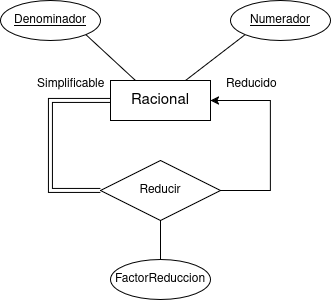
\includegraphics[width=0.5\textwidth]{imagenes/Racional.drawio.png}
  \caption{Diagrama E/R que representa los números racionales.}
\end{figure}

\textbf{Entidades:}
\begin{itemize}
\item Números Racionales
\end{itemize}

\textbf{Atributos:}
\begin{itemize}
\item Números Racionales
  \begin{itemize}
  \item Numerador.
  \item Denominador.
  \item Factor de reducción.
  \end{itemize}
\end{itemize}

\textbf{Relaciones:}
\begin{itemize}
  \item \textbf{Racional - Racional - 1:N}
  \begin{itemize}
    \item \textbf{Racional (Reducido): parcial (0, N)}
    \item \textbf{Racional (Simplificable): total (1, 1)}
    Un racional (reducido) puede tener múltiples racionales (simplificables), pero un racional (simplificable) puede tener un único racional reducido.
  \end{itemize}
\end{itemize}

Para la relación entre números racionales que asocia un racional con su número reducido, se consideró una participación parcial por parte de los números racionales reducidos, pues se menciona que no todos los números racionales son reducidos, y una participación total por parte de los números racionales reducibles, pues se menciona que todos los números racionales tienen un racional reducido.



 \subsection*{b. Modelo E/R para el Modelo E/R}

\textit{}

\addcontentsline{toc}{subsection}{b. Modelo E/R para el Modelo E/R}
\begin{figure}[h]
    \centering
    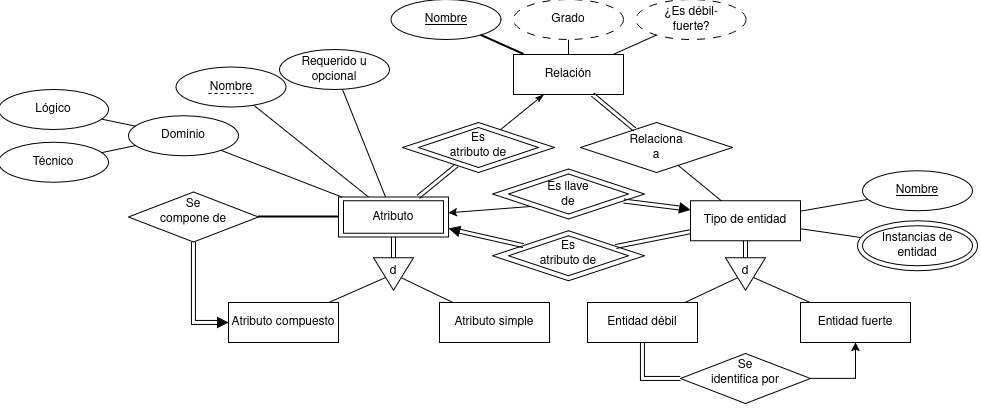
\includegraphics[width=1\linewidth]{imagenes/diagramasER.png}
    \caption{Diagrama Entidad/Relación que representa los conceptos del modelo Entidad/Relación}
\end{figure}
 \subsection*{d. Sistema de Información Geográfica}

\addcontentsline{toc}{subsection}{d. Sistema de Información Geográfica}

\noindent La Secretaría del Medio Ambiente y Recursos Naturales (SEMARNAT) desea crear un SIG (Sistema de Información Geográfica) para acceso público a través de Internet. Se desea crear un modelo E/R atendiendo las siguientes reglas de negocio:

\begin{itemize}
    \item Datos referentes a ríos, afluentes, sistemas montañosos, montañas y municipios donde se localizan.
    
    \item De los ríos se almacenará un identificador del río, nombre, descripción y longitud total. Para cada río, además, se almacenarán los municipios que atraviesa y la longitud del tramo del río para cada municipio bañado.
    
    \item De los municipios se almacenará un identificador para el municipio, nombre y número de habitantes.
    
    \item Los ríos pueden ser afluentes de otros ríos; si es el caso, se desea conocer a cuál río alimentan y el municipio en el que se unen al río del que son afluentes.
    
    \item En cuanto a los sistemas montañosos, se almacenará un código, el nombre, la orientación (norte, sur, este, oeste), la longitud, la altura máxima y los municipios que ocupa. Los sistemas están formados por montañas de las que se almacena un código, un nombre, descripción y altura. Se debe considerar que una montaña sólo pertenecerá a un sistema montañoso. Se requiere almacenar también el municipio o municipios en los que se encuentra, ya que hay casos en los que una montaña es compartida por varios municipios.
    
    \item Las montañas además pueden tener un origen volcánico o de plegamiento. En el caso de que su origen sea volcánico, se desea almacenar el tipo de volcán y si es de plegamiento, se almacenará el periodo geológico de dicho plegamiento.
    
    \item Algunos ríos y montañas son elementos geológicos monitoreados por satélite. De dichos elementos se desea almacenar la fecha en la que se comienzan a monitorear y el satélite que realiza el seguimiento. Un satélite puede monitorear varios elementos. De los satélites se desea almacenar su identificador.
\end{itemize}



\begin{figure}[H]
    \centering
    
\includegraphics[width=1\linewidth]{imagenes/Sistema Geográfico.drawio.png}
    \caption{Diagrama Entidad/Relación que representa un Sistema de Información Geográfica}
\end{figure}

\begin{itemize}
    \item \textbf{Entidades regulares (fuertes)}
    \begin{itemize}
        \item \textbf{Río}
        \begin{itemize}
            \item \underline{\texttt{IdRio}} 
            \item Nombre
            \item Descripcion
            \item LongitudTotal
        \end{itemize}

        \item \textbf{Municipio}
        \begin{itemize}
            \item \underline{{IdMunicipio}} 
            \item Nombre
            \item NumHabitantes
        \end{itemize}

        \item \textbf{Sistema montañoso}
        \begin{itemize}
            \item \underline{{Código}} 
            \item Nombre
            \item Longitud
            \item Orientacion (Atributo multivaluado)
            \item AlturaMaxima (Atributo derivado)
        \end{itemize}

        \item \textbf{Montaña} (Superentidad de la especialización)
        \begin{itemize}
            \item \underline{{Código}} 
            \item Nombre
            \item Descripcion
            \item Altura
        \end{itemize}

        \item \textbf{Satélite}
        \begin{itemize}
            \item \underline{{IdSatelite}} 
            \item Nombre
            \item Descripcion
        \end{itemize}
    \end{itemize}

    \item \textbf{Entidades débiles}
    \begin{itemize}
        \item \textbf{Afluencia}
        \begin{itemize}
            \item Asociada de forma total a las relaciones \texttt{Desembocar}, \texttt{Alimentar} y \texttt{Ocurrir}.
        \end{itemize}
    \end{itemize}

    \item \textbf{Atributos descriptivos de la relación}
    \begin{itemize}
        \item \textbf{Atravesar:} \texttt{LongitudTramo}
        \item \textbf{Monitorear:} \texttt{FechaInicio}
    \end{itemize}
\end{itemize}

\textbf{Consideraciones}
\begin{enumerate}
    \item Dado que solamete algunos ríos y montañas son monitoreados por satélite, y al tratarse de dos tipos de entidades con atributos y llaves distintas, se definió una categoría \texttt{ElemMonitoreado}. Lo cual garantiza que la herencia de atributos sea selectiva y que la relación \texttt{Monitorear} se asocie únicamente a los elementos geológicos registrados.
    
    \item Se definió una especialización por disyunción parcial para la entidad \texttt{Montaña}, dividida en \texttt{Volcánica} y \texttt{Plegamiento}. Esto debido a que una montaña puede ser de origen volcánico o de plegamiento, perteneciendo a una sola de estas subclases si es su causa de origen.

    \item \texttt{LongitudTramo} se colocó como un atributo descriptivo de la relación \texttt{atravesar}, ya que la longitud de un río dentro de un municipio depende de las dos entidades.
    
    \item \texttt{FechaInicio} se asignó como atributo descriptivo de la relación \texttt{Monitorear}, representando el momento exacto en que un satélite específico comienza el seguimiento de un elemento geológico específico.
\end{enumerate}

\textbf{Relaciones, Cardinalidad y Participación}

\begin{itemize}
    \item \textbf{ATRAVESAR} Río - Municipio -- $N:M$
    \begin{itemize}

        \item \textbf{Río:} Parcial $(0,N)$
        \item \textbf{Municipio:} Parcial $(0,N)$
        \item Un río puede atravesar varios municipios, mientras que un municipio puede ser atravesado por varios ríos. No todo río atraviesa uno o varios municipios, ni todo municipio es atravesado por un río. 
    \end{itemize}

    \item \textbf{DESEMBOCAR} Río - Afluencia - $1:1$
    \begin{itemize}
        \item \textbf{Río:} Parcial $(0,1)$
        \item \textbf{Afluencia:} Total $(1,1)$
        \item Un río si es afluente esemboca en un único punto registrado de afluencia, pero no todos los ríos son afluentes. 
    \end{itemize}

    \item \textbf{ALIMENTAR} Afluencia - Río - $N:1$
    \begin{itemize}
        \item \textbf{Afluencia:} Total $(1,1)$
        \item \textbf{Río:} Parcial $(0,N)$
        \item Una afluencia alimenta a un único río receptor. En cambio, un río puede recibir agua de múltiples ríos afluentes o no recibir de ninguno.
    \end{itemize}

    \item \textbf{OCURRIR} Afluencia - Municipio - $N:1$
    \begin{itemize}
  
        \item \textbf{Afluencia:} Total $(1,1)$
        \item \textbf{Municipio:} Parcial $(0,N)$
        \item Cada punto de afluencia ocurre dentro de un único municipio. Un municipio puede recibir varias afluencias o no recibir ninguna.
    \end{itemize}

    \item \textbf{OCUPAR} Sistema montañoso - Municipio - $N:M$
    \begin{itemize}
        
        \item \textbf{Sistema montañoso:} Parcial $(0,N)$
        \item \textbf{Municipio:} Parcial $(0,N)$
        \item Un sistema montañoso puede ocupar varios municipios, y un municipio puede ser ocupado por más de un sistema montañoso.
    \end{itemize}

    \item \textbf{FORMAR} Sistema montañoso - Montaña - $1:N$
    \begin{itemize}
        
        \item \textbf{Sistema montañoso:} Parcial $(0,N)$
        \item \textbf{Montaña:} Total $(1,1)$
        \item Un sistema montañoso está integrado por varias montañas  y cada montaña pertenece obligatoriamente a un único sistema montañoso.
    \end{itemize}

    \item \textbf{UBICAR} Municipio - Montaña - $N:M$
    \begin{itemize}
        
        \item \textbf{Municipio:} Parcial $(0,N)$
        \item \textbf{Montaña:} Parcial $(0,N)$
        \item Una montaña puede ubicarse entre uno o varios municipios, y un municipio puede albergar a múltiples montañas.
    \end{itemize}

    \item \textbf{MONITOREAR} Satélite - ElemMonitoreado - $1:N$
    \begin{itemize}
        
        \item \textbf{Satélite:} Parcial $(0,N)$
        \item \textbf{ElemMonitoreado:} Total $(1,1)$
        \item Un satélite puede monitorear varios elementos geológicos. Cada elemento monitoreado es seguido por un solo satélite. 
    \end{itemize}
\end{itemize}

%\nocite{*} 
%\printbibliography[title={Referencias}]

\end{document}
